\documentclass[]{article}

%These tell TeX which packages to use.
\usepackage{array,epsfig}
\usepackage{amsmath}
\usepackage{amsfonts}
\usepackage{amssymb}
\usepackage{amsxtra}
\usepackage{amsthm}
% \usepackage{mathrsfs}
\usepackage{color}
\usepackage{hyperref}
\usepackage{enumitem}
\usepackage{float}
\usepackage{bm}
%Here I define some theorem styles and shortcut commands for symbols I use often
\theoremstyle{definition}
\newtheorem{defn}{Definition}
\newtheorem{thm}{Theorem}
\newtheorem{cor}{Corollary}
\newtheorem*{rmk}{Remark}
\newtheorem{lem}{Lemma}
\newtheorem*{joke}{Joke}
\newtheorem{ex}{Example}
\newtheorem*{soln}{Solution}
\newtheorem{prop}{Proposition}

\newcommand{\lra}{\longrightarrow}
\newcommand{\ra}{\rightarrow}
\newcommand{\surj}{\twoheadrightarrow}
\newcommand{\graph}{\mathrm{graph}}
\newcommand{\bb}[1]{\mathbb{#1}}
\newcommand{\Z}{\bb{Z}}
\newcommand{\Q}{\bb{Q}}
\newcommand{\R}{\bb{R}}
\newcommand{\C}{\bb{C}}
\newcommand{\N}{\bb{N}}
\newcommand{\M}{\mathbf{M}}
\newcommand{\m}{\mathbf{m}}
\newcommand{\MM}{\mathscr{M}}
\newcommand{\HH}{\mathscr{H}}
\newcommand{\Om}{\Omega}
\newcommand{\Ho}{\in\HH(\Om)}
\newcommand{\bd}{\partial}
\newcommand{\del}{\partial}
\newcommand{\bardel}{\overline\partial}
\newcommand{\textdf}[1]{\textbf{\textsf{#1}}\index{#1}}
\newcommand{\img}{\mathrm{img}}
\newcommand{\ip}[2]{\left\langle{#1},{#2}\right\rangle}
\newcommand{\inter}[1]{\mathrm{int}{#1}}
\newcommand{\exter}[1]{\mathrm{ext}{#1}}
\newcommand{\cl}[1]{\mathrm{cl}{#1}}
\newcommand{\ds}{\displaystyle}
\newcommand{\vol}{\mathrm{vol}}
\newcommand{\cnt}{\mathrm{ct}}
\newcommand{\osc}{\mathrm{osc}}
\newcommand{\LL}{\mathbf{L}}
\newcommand{\UU}{\mathbf{U}}
\newcommand{\support}{\mathrm{support}}
\newcommand{\AND}{\;\wedge\;}
\newcommand{\OR}{\;\vee\;}
\newcommand{\Oset}{\varnothing}
\newcommand{\st}{\ni}
\newcommand{\wh}{\widehat}

%Pagination stuff.
\setlength{\topmargin}{-.3 in}
\setlength{\oddsidemargin}{0in}
\setlength{\evensidemargin}{0in}
\setlength{\textheight}{9.in}
\setlength{\textwidth}{6.5in}
\pagestyle{empty}
\usepackage{braket}
\usepackage{natbib}
\usepackage{bibentry}
\bibliographystyle{plainnat}



\begin{document}

\begin{center}
  {FOR 1807 Winter School 2018 Marburg}\\
  \textbf{Exact Diagonalization hands-on
    session}\\ %You should put your name here
  Exercise sheet\\
  Alexander Wietek, Andreas Honecker% You should write the date here.
\end{center}

\vspace{0.2 cm}

% \subsection{Overview}
In the following exercises we will make use of the scripts
\texttt{hamiltonian\_tfi.py}, \texttt{hamiltonian\_hb\_staggered.py}
and \texttt{hamiltonian\_hb\_xxz.py}.  The three files contain each
contain a function \texttt{get\_hamiltonian\_sparse} which creates the
Hamiltonian matrix in a sparse matrix format. The following
Hamiltonians are given
\begin{itemize}
\item \texttt{hamiltonian\_tfi.py}: The \textit{Transverse Field
    Ising} model,
  \begin{equation}
    \label{eq:tfi}
    H = -J\sum\limits_{\langle i , j \rangle} \sigma^z_i\sigma^z_j - h_x \sum\limits_{i}\sigma^x,
  \end{equation}
  where $\sigma^z$ and $\sigma^x$ are the Pauli matrices, on a
  one-dimensional chain lattice (with periodic boundary conditions).
  This model does not conserve total $S^z$. Momentum conservation is
  not implemented.
\item \texttt{hamiltonian\_hb\_staggered.py}: The \textit{Heisenberg
    model in a staggered magnetic field} ,
  \begin{equation}
    \label{eq:hb_stag}
    H = J\sum\limits_{\langle i , j \rangle} \mathbf{S}_i\cdot\mathbf{S}_j + h_S \sum\limits_{i}(-1)^iS^z,
  \end{equation}
  one-dimensional chain lattice (with periodic boundary conditions).
  This model does conserve total $S^z$. Momentum conservation is not
  implemented.
\item \texttt{hamiltonian\_hb\_xxz.py}: The \textit{Heisenberg model
    with Ising anisotropy} ,
  \begin{equation}
    \label{eq:hb_xxz}
    H = J\sum\limits_{\langle i , j \rangle} \left[S^z_iS^z_j +
      (1+\Delta)\left(S^x_iS^x_j + S^y_iS^y_j\right)\right]
  \end{equation}
  one-dimensional chain lattice (with periodic boundary conditions).
  This model does conserve total $S^z$. Momentum conservation is
  implemented.
\end{itemize}
An example how to use these functions for computations can be found in
the file \texttt{example\_groundstate\_energy.py}. Internally, spin
states are encoded in a binary representation, for example
\begin{equation}
  \ket{\uparrow\downarrow\uparrow \uparrow} = (1011)_2 = 11.
\end{equation}
The scripts are kept short, to be easily accesible. Please just ask if
you have any questions how they work.

\begin{center}
  Have fun with the exercises!
\end{center}


\newpage
\subsection*{Exercise 1: Impementing a Hamiltonian, computing static
  correlations (basic)}
\begin{enumerate}[label=(\alph*)]
\item We consider the transverse field Ising model as defined by
  Eq.~\ref{eq:tfi}. Use the script \texttt{hamiltonian\_tfi.py} to
  compute lowest 10 eigenvalues for $J=1$ and for a range of values
  $h_x$ from $0$ to $2$ for a chain of length $L=12$. Plot the
  excitation energies as a function of $h_x$. The model has a phase
  transition from a ferromagnetic phase to a paramagnetic phase at
  $h_x=1$.  Can you detect the phase transition by investigating the
  energy spectra?
  \paragraph{Result:}
  The energies as a function of the transverse field are shown in the
  following plot:
  \begin{figure}[H]
    \centering
    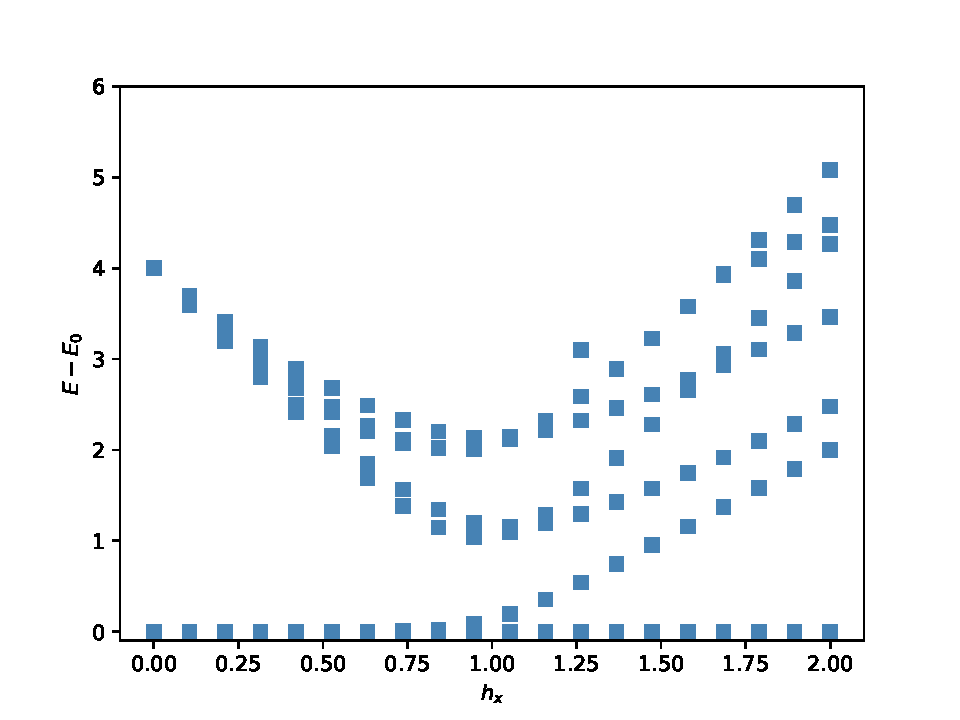
\includegraphics[width=0.5\textwidth]{spectra_tfi_12.pdf}
  \end{figure}

  \paragraph{Hints:}
  \begin{itemize}
  \item Use the function \texttt{get\_hamiltonian\_sparse()} to create
    the sparse matrix of the Hamiltonian for a given $h_x$
  \item Create a scipy sparse matrix and compute low lying eigenvalues
    as shown in \texttt{example\_groundstate\_energy.py}.
  \item Perform the above steps for multiply values of $h_x$ and plot
    the results using matplotlib.
  \end{itemize}

  
\item Alter the script \texttt{hamiltonian\_tfi.py} to create the
  Hamiltonian of the spin-$1/2$ Heisenberg model,
  \begin{equation}
    \label{eq:hb}
    H = J\sum\limits_{\langle i , j \rangle} \mathbf{S}_i\cdot\mathbf{S}_j,
  \end{equation}
  and compute its ground state energy for a chain of length $L=12$.
  Cross check the ground state energy with the script
  \texttt{hamiltonian\_hb\_staggered.py} for total $S^z=0$.

  As a supplement, investigate the behaviour of the ground state
  energy as a function of the system size $L$ and check out the
  convergence to
  \begin{equation*}
    E_0/L = -\log{2} + 1/4. 
  \end{equation*}
  \paragraph{Result:}
  The ground state energy for $L=12$ as described above is given by
  $$E_0/L = -0.44894924 $$
  \paragraph{Hints:}
  \begin{itemize}
  \item We have to modify \texttt{get\_hamiltonian\_sparse()} in the
    file \texttt{hamiltonian\_tfi.py}
  \item Replace lines 48-66 in this file by the implementation of the
    Heisenberg bond in the file\\
    \texttt{hamiltonian\_hb\_staggered.py}, lines 79-104 (omitting the
    staggered field).
  \end{itemize}

\item Compute the ground state spin correlations
  $\braket{0|S^z_0S^z_r|0}$ and
  $\braket{0|\mathbf{S}_0\cdot\mathbf{S}_r|0}$ of the spin-$1/2$
  Heisenberg model in Eq.~\ref{eq:hb} for a chain of length
  $L=12$. Check, whether
  $$\braket{0|\mathbf{S}_0\cdot\mathbf{S}_r|0} = 3\braket{0|S^z_0S^z_r|0}.$$
  This equality holds due to $\mathrm{SU}(2)$ rotational symmetry of
  the ground state $\ket{0}$.
  \paragraph{Result:}
  The ground state correlations as descibed above are shown in the
  following plot:
  \begin{figure}[H]
    \centering
    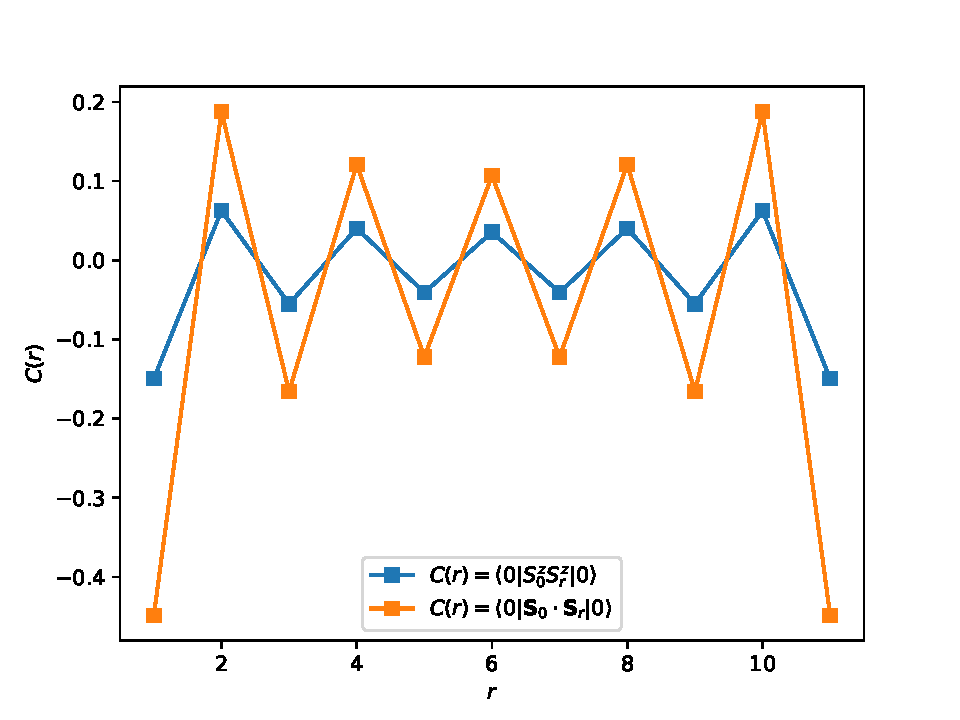
\includegraphics[width=0.5\textwidth]{correlations_hbchain_12.pdf}
  \end{figure}
  \paragraph{Hints:}
  \begin{itemize}
  \item Create matrices for the operators $S^z_0S^z_r$ and
    $\mathbf{S}_0\cdot\mathbf{S}_r$. This can be done analogously to
    creating the Hamiltonian.
  \item Use scipy and numpy multiplication routines to evaluate
    $\braket{0|S^z_0S^z_r|0}$ and
    $\braket{0|\mathbf{S}_0\cdot\mathbf{S}_r|0}$ for different values
    of $r$.
  \end{itemize}
\end{enumerate}

\newpage
\subsection*{Exercise 2: Hamiltonian symmetries (advanced)}
In this exercise we investigate the Heisenberg XXZ model
Eq.~\ref{eq:hb_xxz}. This model has a discrete translational symmetry
$T:\ket{\sigma_1, \sigma_2, \ldots, \sigma_L} \mapsto \ket{\sigma_L,
  \sigma_1, \ldots, \sigma_{L-1}}$. Hence, a symmetrized basis with
fixed momentum $2\pi k / L$ can be chosen. The script
\texttt{hamiltonian\_hb\_xxz.py} creates the Hamiltonian of the
Heisenberg model with Ising anisotropy as defined in
Eq.~\ref{eq:hb_xxz} in the basis of momentum eigenstates.
$$
\ket{\bm{\sigma}^k} = \frac{1}{N_{\bm{\sigma}}}
\sum_{n=0}^{L-1}\text{e}^{i2\pi k n / L}T^n\ket{\bm{\sigma}},
$$
where $N_{\bm{\sigma}}$ denotes the normalization constant of the
symmetrized state $\ket{\bm{\sigma}^k}$.  $k$ can be
chosen as a parameter and acts as a label for the different momentum
sectors.
\begin{enumerate}
\item Compute the lowest 10 eigenvalues of the Hamiltonian for each
  $k = 0, \ldots, L=16$ and plot the energies as a function of
  momentum for the isotropic Heisenberg case.
  \paragraph{Result:}
  The momentum resoved eigenvalues for $L=16$ are shown in the
  following plot:
  \begin{figure}[H]
    \centering
    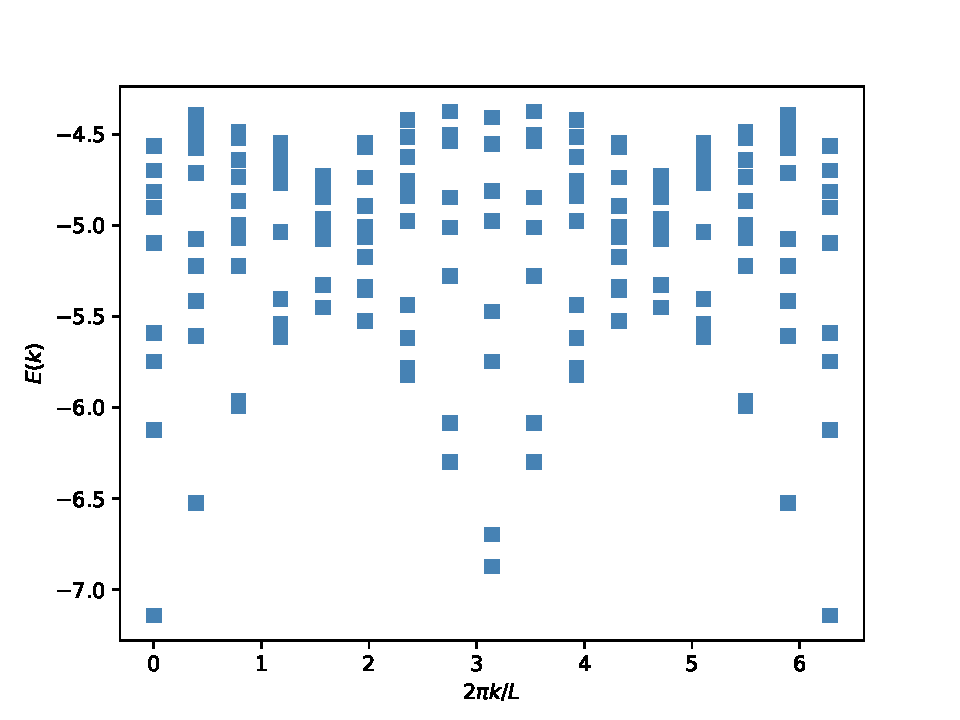
\includegraphics[width=0.5\textwidth]{spectra_hbchain_16_kresolved.pdf}
  \end{figure}
  \paragraph{Hints:}
  \begin{itemize}
  \item Use the function \texttt{get\_hamiltonian\_sparse()} to create
    the sparse matrix of the Hamiltonian for a given momentum $k$
  \item Create a scipy sparse matrix and compute low lying eigenvalues
    as shown in \texttt{example\_groundstate\_energy.py}.
  \item Perform the above steps for multiply values of $k$ and plot
    the results using matplotlib. Notice that the actual momentum is
    given by $2\pi k /L$
  \item If you want to understand in detail, how the symmetrized basis
    for translational symmetry is built up, have a look at the
    implementation \texttt{hamiltonian\_hb\_xxz.py} and \cite{weise}.
  \end{itemize}
\item We are now going to implement a spinflip symmetry for the
  transverse Field Ising model in Eq.~\ref{eq:tfi}. The spinflip
  symmetry flips all spins at all sites,
  $S: \ket{\sigma_1, \sigma_2, \ldots, \sigma_L} \mapsto
  \ket{-\sigma_1, -\sigma_2, \ldots, -\sigma_L}$. Check that this
  operator commutes with the Hamiltonian, $[H,S]$. The spinflip
  symmetry is simpler to utilize than translational symmetries.

  \paragraph{Evaluating matrix elements in the symmetrized basis:}
  We will now describe how to evaluate the matrix elements in the
  spinflip symmetrized basis. The symmetrized basis states given by
  $$ \ket{\bm{\sigma}^{\gamma}} = \frac{1}{\sqrt{2}}
  \left( \ket{\bm{\sigma}} + \gamma S\ket{\bm{\sigma}} \right). $$
  $\ket{\bm{\sigma}^{\gamma}}$ denote the symmetrized states in the even
  ($\gamma=1$) and odd ($\gamma=-1$) representation of the spinflip
  symmetry. Our goal for now is to evaluate matrix elements of the
  form
  $$\braket{\bm{\tau}^{\gamma}| H_k | \bm{\sigma}^{\gamma}}.$$
  To represent the symmetrized state on the computer we choose
  $\ket{\tilde{\bm{\sigma}}} = \min( \ket{\bm{\sigma}},
  S\ket{\bm{\sigma}})$ and call this state a representative.  If we
  apply an offdiagonal, non-branching term (i.e. one spin
  configuration is only mapped to one single other configuration),
  $$H_k\ket{\tilde{\bm{\sigma}}} = c_k\ket{\bm{\tau}},$$
  the state $\ket{\bm{\tau}}$ need not necessarily be a
  representative.  Put differntly, $S\ket{\bm{\tau}}$ could be smaller
  than $\ket{\bm{\tau}}$. Let again
  $H_k\ket{\tilde{\bm{\sigma}}} = c_k\ket{\bm{\tau}}$. The matrix
  element between two representatives is given by
  \[
    \braket{\tilde{\bm{\tau}}^{\gamma}| H_k | \bm{\tilde{\sigma}}^{\gamma}}=
    \begin{cases}
      c_k \text { if } \ket{\bm{\tau}} = \ket{\tilde{\bm{\tau}}} \\
      \gamma c_k \text { if } \ket{\bm{\tau}} = S\ket{\tilde{\bm{\tau}}}
    \end{cases}
  \]
  Check this equation!

  \paragraph{How to implenent spinflip symmetry, step by step:}
  Spinflip symmetry can be implemented in a manner analogous to the
  implementation of translational symmetry in
  \texttt{hamiltonian\_hb\_xxz.py}.
  \begin{itemize}
  \item Start with the function \texttt{get\_hamiltonian\_sparse()}
    from \texttt{hamiltonian\_tfi.py} and add an additional parameter
    \texttt{gamma} which should be $\pm 1$, depending whether we choose
    the even/odd representation.
  \item define a function \texttt{flip()} that flips all the spins for
    a given spin configuration
  \item define a function \texttt{get\_representative()} that, for a
    given state $\ket{\bm{\sigma}}$ returns $\ket{\bm{\sigma}}$ if
    $\ket{\bm{\sigma}} < S\ket{\bm{\sigma}}$ and $S\ket{\bm{\sigma}}$
    else. You can use the function \texttt{flip()}. This function
    should also return as a second value \texttt{gamma} if the flipped
    state is returned and $1$ else.
  \item We need to create a list of representatives. To do so run
    through all spin configurations and save those who are
    representatives to a list.
  \item Instead of looping over all spin configurations, we now only
    loop over the representatives to create the Hamiltonian. This
    yields the dimensional reduction.
  \item The evaluation of diagonal elements remains unaltered.
  \item The off-diagonal elements need to be computed differently.
    After the transverse field bond is applied, we need to find the
    representative of this state. Use the function
    \texttt{get\_representative()} to do so. This function should also
    return \texttt{gamma} if the state has been flipped.
  \item The coefficient is now given by $\texttt{gamma} \cdot h_x$.
    The column and row indices are determined by the location of both
    states in the list of representatives.
  \end{itemize}
  Follwing these instructions, we can now compute eigenvalues of the
  Hamiltonian in the even and odd spinflip sector. Compute the lowest
  10 eigenvalues for a range $h_x=0,\ldots,2$ and both symmetry
  sectors. Plot the excitation energies and compare to exercise
  1a). Why are the even and the odd sector degenerate in the
  ferromagnetic case?
  \newpage
  \paragraph{Result:}
  The excitation energies for the even/odd symmetry sectors are shown
  in the following figure:
  \begin{figure}[H]
    \centering
    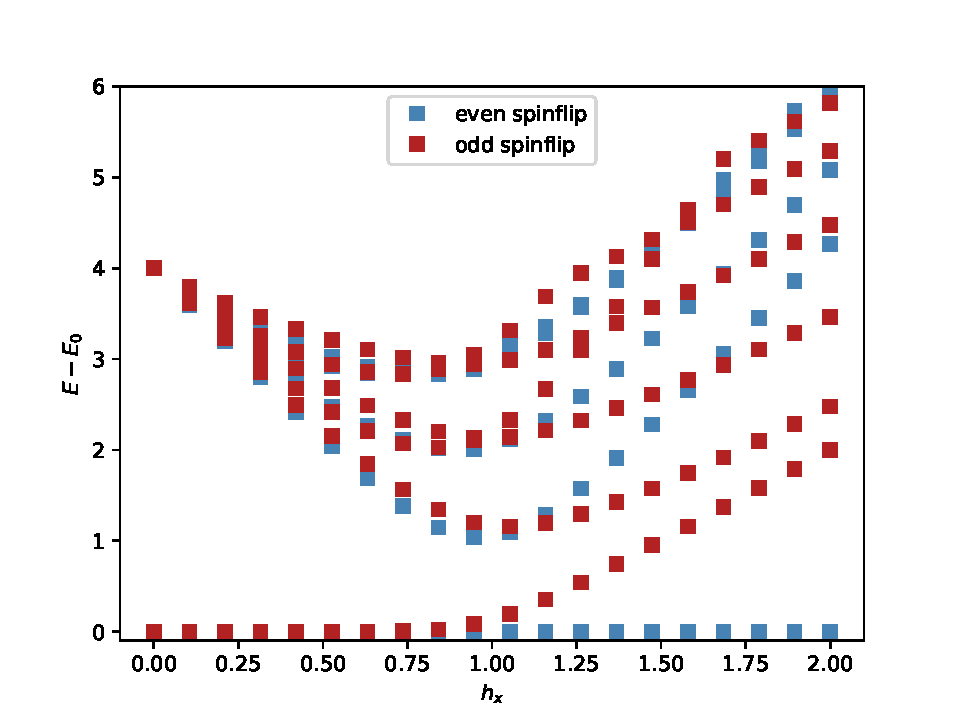
\includegraphics[width=0.5\textwidth]{spectra_tfi_12_spinflip.pdf}
  \end{figure}  
\end{enumerate}

% \newpage

% \subsection*{Exercise 3: Computing dynamical correlations functions}
% In this exercise we compute the ground state Greeen's function,
% \begin{equation}
%   \label{eq:greensfunction}
%   G^{zz}(\mathbf{q}, z) = \braket{0|S^{\dagger}(\mathbf{q}) 
%     \frac{1}{z-H}S(\mathbf{q})|0}, \text{ where } z = \omega+i\eta,
% \end{equation}
% and the corresponding dynamical spin structure factor
% \begin{equation}
%   \label{eq:dynspin}
%   S^{zz}(\mathbf{q}, \omega) = -\frac{1}{\pi}\lim_{\eta \rightarrow 0}\text{Im}
%   G^{zz}(\mathbf{q}, \omega + i\eta),
% \end{equation}
% where
% $$S^z(\mathbf{q}) = \frac{1}{\sqrt{L}}\sum\limits_{\mathbf{r}} e^{-i\mathbf{q}{\mathbf{r}}}S^z.$$
% We will compute these quantities for the isotropic Heisenberg chain,
% as in Eq.~\ref{eq:hb_stag} with $h_s=0$.  $L$ denotes the length of
% the chain whose discrete momenta are given by
% $\mathbf{q} = 2\pi/L \cdot 0, 2\pi/L \cdot 1, \ldots, 2\pi/L \cdot
% (L-1)$.  The Hamiltonian $H$ can be created using the script
% \texttt{hamiltonian\_hb\_staggered.py}.
% \begin{enumerate}
% \item (basic) Fix a small but finite $\eta$. Compute the Green's
%   function Eq.~\ref{eq:greensfunction} and the dynamical spin
%   structure factor Eq.~\ref{eq:dynspin} by creating a dense matrix $H$
%   of the Hamiltonian and inverting $(z - H)$ numerically for small
%   system sizes.
% \item (advanced) The Green's function can be evaluated without fully
%   inverting the matrix $(z-H)$ using the \textit{continuous fraction
%     expansion},
%   \begin{equation}
%     \label{eq:contfrac}
%     G^{zz}(\mathbf{q}, z) =
%     \frac{\braket{0|S^{\dagger}(\mathbf{q})S(\mathbf{q})|0}}
%     {z - \alpha_0- \frac{\beta_1^2}{z - \alpha_1 - \frac{\beta_2^2}{z-\cdots}}}
%   \end{equation}
%   Here, $\alpha_n$, $\beta_n$ are given by the Lanczos recursion,
%   \begin{align*}
%     \ket{v_{n+1}} &= \beta_{n+1}^{-1}\left[(H-\alpha_n)\ket{v_n} - \beta_n \ket{v_{n-1}}\right] \\
%     \alpha_n &= \braket{v_n|H|v_n} \\
%     \beta_{n+1} &= \parallel(H-\alpha_n)\ket{v_n} - \beta_n \ket{v_{n-1}}\parallel,
%   \end{align*}
%   with starting vector $\ket{v_0} = S(\mathbf{q})\ket{0}$. A basic
%   implementation of the Lanczos recursion creating the coefficients
%   $\alpha_n$ and $\beta_n$ can be found in the file
%   \texttt{algorithm\_lanczos.py}. Compare the results from continuous
%   fraction expansion to the results from full inversion. For details
%   on the continuous fraction expansion see e.g. \cite{koch20118}.
% \end{enumerate}

\bibliography{exercises}
\end{document}


